\documentclass{article}
\usepackage{lmodern}
\usepackage[T1]{fontenc}
\usepackage{shapepar}
\usepackage{microtype}
\usepackage{lipsum}
\usepackage{pgfplots}
\pgfplotsset{compat=1.9}
\usepackage{tikz}
\usetikzlibrary{calc,fit,intersections,folding}
\usepackage{pstricks-add}
\usetikzlibrary{arrows.meta,angles,arrows,quotes,backgrounds}

\newcommand{\tubecolor}{blue}
\newcommand{\thickness}{0.5mm}
\newcommand{\n}{2mm}

\begin{document}
\begin{center}
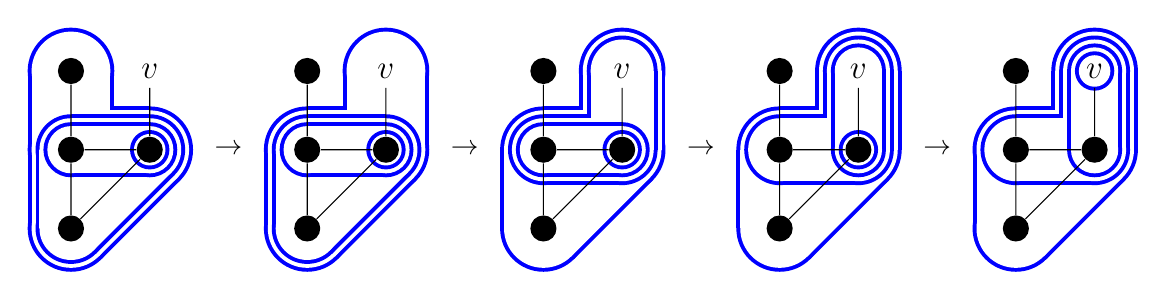
\begin{tikzpicture}
    \thispagestyle{empty}
    \begin{scope}
        \node[fill] (A) at (0,0) [circle] {};
        \node[fill] (B) at (0,-1) [circle] {};
        \node[fill] (C) at (0,-2) [circle] {};
        \node[fill] (D) at (1,-1) [circle] {};
        \node (v) at (1,0) {\large$v$};
    
        \draw (A) -- (B) -- (C) -- (D) -- (v) (B) -- (D);
        %Tube ABCD:
        \begin{scope}[on background layer]
            \fill[\tubecolor] (A) circle (\n + 7*\thickness);
            \fill[\tubecolor] (B) circle (\n + 7*\thickness);
            \fill[\tubecolor] (D) circle (\n + 7*\thickness);
            \fill[\tubecolor] (C) circle (\n + 7*\thickness);
            \draw[\tubecolor] [line width = 2*(\n + 7*\thickness)] (A.center) -- (B.center);
            \draw[\tubecolor] [line width = 2*(\n + 7*\thickness)] (C.center) -- (D.center);
            \draw[\tubecolor] [line width = 2*(\n + 7*\thickness)] (B.center) -- (D.center);
            \draw[\tubecolor] [line width = 2*(\n + 7*\thickness)] (B.center) -- (C.center);
            
            \fill[white] (A) circle (\n + 6*\thickness);
            \fill[white] (B) circle (\n + 6*\thickness);
            \fill[white] (D) circle (\n + 6*\thickness);
            \fill[white] (C) circle (\n + 6*\thickness);
            \draw[white] [line width = 2*(\n + 6*\thickness)] (A.center) -- (B.center);
            \draw[white] [line width = 2*(\n + 6*\thickness)] (C.center) -- (D.center);
            \draw[white] [line width = 2*(\n + 6*\thickness)] (B.center) -- (D.center);
            \draw[white] [line width = 2*(\n + 6*\thickness)] (B.center) -- (C.center);
        \end{scope}
        %Tube BCD:
        \begin{scope}[on background layer]
            \fill[\tubecolor] (B) circle (\n + 5*\thickness);
            \fill[\tubecolor] (D) circle (\n + 5*\thickness);
            \fill[\tubecolor] (C) circle (\n + 5*\thickness);
            \draw[\tubecolor] [line width = 2*(\n + 5*\thickness)] (C.center) -- (D.center);
            \draw[\tubecolor] [line width = 2*(\n + 5*\thickness)] (B.center) -- (D.center);
            \draw[\tubecolor] [line width = 2*(\n + 5*\thickness)] (B.center) -- (C.center);
            
            \fill[white] (B) circle (\n + 4*\thickness);
            \fill[white] (D) circle (\n + 4*\thickness);
            \fill[white] (C) circle (\n + 4*\thickness);
            \draw[white] [line width = 2*(\n + 4*\thickness)] (C.center) -- (D.center);
            \draw[white] [line width = 2*(\n + 4*\thickness)] (B.center) -- (D.center);
            \draw[white] [line width = 2*(\n + 4*\thickness)] (B.center) -- (C.center);
        \end{scope}
        %Tube BD:
        \begin{scope}[on background layer]
            \fill[\tubecolor] (B) circle (\n + 3*\thickness);
            \fill[\tubecolor] (D) circle (\n + 3*\thickness);
            \draw[\tubecolor] [line width = 2*(\n + 3*\thickness)] (B.center) -- (D.center);
            
            \fill[white] (B) circle (\n + 2*\thickness);
            \fill[white] (D) circle (\n + 2*\thickness);
            \draw[white] [line width = 2*(\n + 2*\thickness)] (B.center) -- (D.center);
        \end{scope}
        %Tube D:
        \begin{scope}[on background layer]
            \fill[\tubecolor] (D) circle (\n + 1*\thickness);
            
            \fill[white] (D) circle (\n + 0*\thickness);
        \end{scope}
        \node at (2,-1) {$\to$};
    \end{scope}
    \begin{scope}[xshift = 3cm]
        \node[fill] (A) at (0,0) [circle] {};
        \node[fill] (B) at (0,-1) [circle] {};
        \node[fill] (C) at (0,-2) [circle] {};
        \node[fill] (D) at (1,-1) [circle] {};
        \node (v) at (1,0) {\large$v$};
    
        \draw (A) -- (B) -- (C) -- (D) -- (v) (B) -- (D);
        %Tube BCDv:
        \begin{scope}[on background layer]
            \fill[\tubecolor] (v) circle (\n + 7*\thickness);
            \fill[\tubecolor] (B) circle (\n + 7*\thickness);
            \fill[\tubecolor] (D) circle (\n + 7*\thickness);
            \fill[\tubecolor] (C) circle (\n + 7*\thickness);
            \draw[\tubecolor] [line width = 2*(\n + 7*\thickness)] (D.center) -- (v.center);
            \draw[\tubecolor] [line width = 2*(\n + 7*\thickness)] (C.center) -- (D.center);
            \draw[\tubecolor] [line width = 2*(\n + 7*\thickness)] (B.center) -- (D.center);
            \draw[\tubecolor] [line width = 2*(\n + 7*\thickness)] (B.center) -- (C.center);
            
            \fill[white] (v) circle (\n + 6*\thickness);
            \fill[white] (B) circle (\n + 6*\thickness);
            \fill[white] (D) circle (\n + 6*\thickness);
            \fill[white] (C) circle (\n + 6*\thickness);
            \draw[white] [line width = 2*(\n + 6*\thickness)] (D.center) -- (v.center);
            \draw[white] [line width = 2*(\n + 6*\thickness)] (C.center) -- (D.center);
            \draw[white] [line width = 2*(\n + 6*\thickness)] (B.center) -- (D.center);
            \draw[white] [line width = 2*(\n + 6*\thickness)] (B.center) -- (C.center);
        \end{scope}
        %Tube BCD:
        \begin{scope}[on background layer]
            \fill[\tubecolor] (B) circle (\n + 5*\thickness);
            \fill[\tubecolor] (D) circle (\n + 5*\thickness);
            \fill[\tubecolor] (C) circle (\n + 5*\thickness);
            \draw[\tubecolor] [line width = 2*(\n + 5*\thickness)] (C.center) -- (D.center);
            \draw[\tubecolor] [line width = 2*(\n + 5*\thickness)] (B.center) -- (D.center);
            \draw[\tubecolor] [line width = 2*(\n + 5*\thickness)] (B.center) -- (C.center);
            
            \fill[white] (B) circle (\n + 4*\thickness);
            \fill[white] (D) circle (\n + 4*\thickness);
            \fill[white] (C) circle (\n + 4*\thickness);
            \draw[white] [line width = 2*(\n + 4*\thickness)] (C.center) -- (D.center);
            \draw[white] [line width = 2*(\n + 4*\thickness)] (B.center) -- (D.center);
            \draw[white] [line width = 2*(\n + 4*\thickness)] (B.center) -- (C.center);
        \end{scope}
        %Tube BD:
        \begin{scope}[on background layer]
            \fill[\tubecolor] (B) circle (\n + 3*\thickness);
            \fill[\tubecolor] (D) circle (\n + 3*\thickness);
            \draw[\tubecolor] [line width = 2*(\n + 3*\thickness)] (B.center) -- (D.center);
            
            \fill[white] (B) circle (\n + 2*\thickness);
            \fill[white] (D) circle (\n + 2*\thickness);
            \draw[white] [line width = 2*(\n + 2*\thickness)] (B.center) -- (D.center);
        \end{scope}
        %Tube D:
        \begin{scope}[on background layer]
            \fill[\tubecolor] (D) circle (\n + 1*\thickness);
            
            \fill[white] (D) circle (\n + 0*\thickness);
        \end{scope}
        \node at (2,-1) {$\to$};
    \end{scope}
    \begin{scope}[xshift = 6cm]
        \node[fill] (A) at (0,0) [circle] {};
        \node[fill] (B) at (0,-1) [circle] {};
        \node[fill] (C) at (0,-2) [circle] {};
        \node[fill] (D) at (1,-1) [circle] {};
        \node (v) at (1,0) {\large$v$};
    
        \draw (A) -- (B) -- (C) -- (D) -- (v) (B) -- (D);
        %Tube BCDv:
        \begin{scope}[on background layer]
            \fill[\tubecolor] (v) circle (\n + 7*\thickness);
            \fill[\tubecolor] (B) circle (\n + 7*\thickness);
            \fill[\tubecolor] (D) circle (\n + 7*\thickness);
            \fill[\tubecolor] (C) circle (\n + 7*\thickness);
            \draw[\tubecolor] [line width = 2*(\n + 7*\thickness)] (D.center) -- (v.center);
            \draw[\tubecolor] [line width = 2*(\n + 7*\thickness)] (C.center) -- (D.center);
            \draw[\tubecolor] [line width = 2*(\n + 7*\thickness)] (B.center) -- (D.center);
            \draw[\tubecolor] [line width = 2*(\n + 7*\thickness)] (B.center) -- (C.center);
            
            \fill[white] (v) circle (\n + 6*\thickness);
            \fill[white] (B) circle (\n + 6*\thickness);
            \fill[white] (D) circle (\n + 6*\thickness);
            \fill[white] (C) circle (\n + 6*\thickness);
            \draw[white] [line width = 2*(\n + 6*\thickness)] (D.center) -- (v.center);
            \draw[white] [line width = 2*(\n + 6*\thickness)] (C.center) -- (D.center);
            \draw[white] [line width = 2*(\n + 6*\thickness)] (B.center) -- (D.center);
            \draw[white] [line width = 2*(\n + 6*\thickness)] (B.center) -- (C.center);
        \end{scope}
        %Tube BDv:
        \begin{scope}[on background layer]
            \fill[\tubecolor] (B) circle (\n + 5*\thickness);
            \fill[\tubecolor] (D) circle (\n + 5*\thickness);
            \fill[\tubecolor] (v) circle (\n + 5*\thickness);
            \draw[\tubecolor] [line width = 2*(\n + 5*\thickness)] (v.center) -- (D.center);
            \draw[\tubecolor] [line width = 2*(\n + 5*\thickness)] (B.center) -- (D.center);
            
            \fill[white] (B) circle (\n + 4*\thickness);
            \fill[white] (D) circle (\n + 4*\thickness);
            \fill[white] (v) circle (\n + 4*\thickness);
            \draw[white] [line width = 2*(\n + 4*\thickness)] (v.center) -- (D.center);
            \draw[white] [line width = 2*(\n + 4*\thickness)] (B.center) -- (D.center);
        \end{scope}
        %Tube BD:
        \begin{scope}[on background layer]
            \fill[\tubecolor] (B) circle (\n + 3*\thickness);
            \fill[\tubecolor] (D) circle (\n + 3*\thickness);
            \draw[\tubecolor] [line width = 2*(\n + 3*\thickness)] (B.center) -- (D.center);
            
            \fill[white] (B) circle (\n + 2*\thickness);
            \fill[white] (D) circle (\n + 2*\thickness);
            \draw[white] [line width = 2*(\n + 2*\thickness)] (B.center) -- (D.center);
        \end{scope}
        %Tube D:
        \begin{scope}[on background layer]
            \fill[\tubecolor] (D) circle (\n + 1*\thickness);
            
            \fill[white] (D) circle (\n + 0*\thickness);
        \end{scope}
        \node at (2,-1) {$\to$};
    \end{scope}
    \begin{scope}[xshift = 9cm]
        \node[fill] (A) at (0,0) [circle] {};
        \node[fill] (B) at (0,-1) [circle] {};
        \node[fill] (C) at (0,-2) [circle] {};
        \node[fill] (D) at (1,-1) [circle] {};
        \node (v) at (1,0) {\large$v$};
    
        \draw (A) -- (B) -- (C) -- (D) -- (v) (B) -- (D);
        %Tube BCDv:
        \begin{scope}[on background layer]
            \fill[\tubecolor] (v) circle (\n + 7*\thickness);
            \fill[\tubecolor] (B) circle (\n + 7*\thickness);
            \fill[\tubecolor] (D) circle (\n + 7*\thickness);
            \fill[\tubecolor] (C) circle (\n + 7*\thickness);
            \draw[\tubecolor] [line width = 2*(\n + 7*\thickness)] (D.center) -- (v.center);
            \draw[\tubecolor] [line width = 2*(\n + 7*\thickness)] (C.center) -- (D.center);
            \draw[\tubecolor] [line width = 2*(\n + 7*\thickness)] (B.center) -- (D.center);
            \draw[\tubecolor] [line width = 2*(\n + 7*\thickness)] (B.center) -- (C.center);
            
            \fill[white] (v) circle (\n + 6*\thickness);
            \fill[white] (B) circle (\n + 6*\thickness);
            \fill[white] (D) circle (\n + 6*\thickness);
            \fill[white] (C) circle (\n + 6*\thickness);
            \draw[white] [line width = 2*(\n + 6*\thickness)] (D.center) -- (v.center);
            \draw[white] [line width = 2*(\n + 6*\thickness)] (C.center) -- (D.center);
            \draw[white] [line width = 2*(\n + 6*\thickness)] (B.center) -- (D.center);
            \draw[white] [line width = 2*(\n + 6*\thickness)] (B.center) -- (C.center);
        \end{scope}
        %Tube BDv:
        \begin{scope}[on background layer]
            \fill[\tubecolor] (B) circle (\n + 5*\thickness);
            \fill[\tubecolor] (D) circle (\n + 5*\thickness);
            \fill[\tubecolor] (v) circle (\n + 5*\thickness);
            \draw[\tubecolor] [line width = 2*(\n + 5*\thickness)] (v.center) -- (D.center);
            \draw[\tubecolor] [line width = 2*(\n + 5*\thickness)] (B.center) -- (D.center);
            
            \fill[white] (B) circle (\n + 4*\thickness);
            \fill[white] (D) circle (\n + 4*\thickness);
            \fill[white] (v) circle (\n + 4*\thickness);
            \draw[white] [line width = 2*(\n + 4*\thickness)] (v.center) -- (D.center);
            \draw[white] [line width = 2*(\n + 4*\thickness)] (B.center) -- (D.center);
        \end{scope}
        %Tube Dv:
        \begin{scope}[on background layer]
            \fill[\tubecolor] (v) circle (\n + 3*\thickness);
            \fill[\tubecolor] (D) circle (\n + 3*\thickness);
            \draw[\tubecolor] [line width = 2*(\n + 3*\thickness)] (v.center) -- (D.center);
            
            \fill[white] (v) circle (\n + 2*\thickness);
            \fill[white] (D) circle (\n + 2*\thickness);
            \draw[white] [line width = 2*(\n + 2*\thickness)] (v.center) -- (D.center);
        \end{scope}
        %Tube D:
        \begin{scope}[on background layer]
            \fill[\tubecolor] (D) circle (\n + 1*\thickness);
            
            \fill[white] (D) circle (\n + 0*\thickness);
        \end{scope}
        \node at (2,-1) {$\to$};
    \end{scope}
    \begin{scope}[xshift = 12cm]
        \node[fill] (A) at (0,0) [circle] {};
        \node[fill] (B) at (0,-1) [circle] {};
        \node[fill] (C) at (0,-2) [circle] {};
        \node[fill] (D) at (1,-1) [circle] {};
        \node (v) at (1,0) {\large$v$};
    
        \draw (A) -- (B) -- (C) -- (D) -- (v) (B) -- (D);
        %Tube BCDv:
        \begin{scope}[on background layer]
            \fill[\tubecolor] (v) circle (\n + 7*\thickness);
            \fill[\tubecolor] (B) circle (\n + 7*\thickness);
            \fill[\tubecolor] (D) circle (\n + 7*\thickness);
            \fill[\tubecolor] (C) circle (\n + 7*\thickness);
            \draw[\tubecolor] [line width = 2*(\n + 7*\thickness)] (D.center) -- (v.center);
            \draw[\tubecolor] [line width = 2*(\n + 7*\thickness)] (C.center) -- (D.center);
            \draw[\tubecolor] [line width = 2*(\n + 7*\thickness)] (B.center) -- (D.center);
            \draw[\tubecolor] [line width = 2*(\n + 7*\thickness)] (B.center) -- (C.center);
            
            \fill[white] (v) circle (\n + 6*\thickness);
            \fill[white] (B) circle (\n + 6*\thickness);
            \fill[white] (D) circle (\n + 6*\thickness);
            \fill[white] (C) circle (\n + 6*\thickness);
            \draw[white] [line width = 2*(\n + 6*\thickness)] (D.center) -- (v.center);
            \draw[white] [line width = 2*(\n + 6*\thickness)] (C.center) -- (D.center);
            \draw[white] [line width = 2*(\n + 6*\thickness)] (B.center) -- (D.center);
            \draw[white] [line width = 2*(\n + 6*\thickness)] (B.center) -- (C.center);
        \end{scope}
        %Tube BDv:
        \begin{scope}[on background layer]
            \fill[\tubecolor] (B) circle (\n + 5*\thickness);
            \fill[\tubecolor] (D) circle (\n + 5*\thickness);
            \fill[\tubecolor] (v) circle (\n + 5*\thickness);
            \draw[\tubecolor] [line width = 2*(\n + 5*\thickness)] (v.center) -- (D.center);
            \draw[\tubecolor] [line width = 2*(\n + 5*\thickness)] (B.center) -- (D.center);
            
            \fill[white] (B) circle (\n + 4*\thickness);
            \fill[white] (D) circle (\n + 4*\thickness);
            \fill[white] (v) circle (\n + 4*\thickness);
            \draw[white] [line width = 2*(\n + 4*\thickness)] (v.center) -- (D.center);
            \draw[white] [line width = 2*(\n + 4*\thickness)] (B.center) -- (D.center);
        \end{scope}
        %Tube Dv:
        \begin{scope}[on background layer]
            \fill[\tubecolor] (v) circle (\n + 3*\thickness);
            \fill[\tubecolor] (D) circle (\n + 3*\thickness);
            \draw[\tubecolor] [line width = 2*(\n + 3*\thickness)] (v.center) -- (D.center);
            
            \fill[white] (v) circle (\n + 2*\thickness);
            \fill[white] (D) circle (\n + 2*\thickness);
            \draw[white] [line width = 2*(\n + 2*\thickness)] (v.center) -- (D.center);
        \end{scope}
        %Tube v:
        \begin{scope}[on background layer]
            \fill[\tubecolor] (v) circle (\n + 1*\thickness);
            
            \fill[white] (v) circle (\n + 0*\thickness);
        \end{scope}
    \end{scope}
\end{tikzpicture}
\end{center}

\end{document}